\section{Resumen}

Este trabajo consiste en la realizaci\'on de un filtro que cumpla con las siguientes especificaciones pautadas:

	\begin{table}[H]
	\centering
	\begin{tabular}{c c}
		\hline
		$f_a$ & $10kHz$\\
		$f_p$ & $13,75kHz$\\
		$A_a$ & $45dB$\\
		$A_p$ & $1dB$\\
		Rango din\'amico & $45dB$\\	
		\hline
	\end{tabular}
	\caption{Especificaciones del filtro pasa altos a realizar.}
	\label{especificaciones}
\end{table}

\section{Introducci\'on te\'orica}

\section{Dise\~no del filtro}

\subsection{Obtenci\'on de polos, ceros y Q a partir de la aproximaci\'on de Legendre}

La finalidad de implementar un filtro a partir de una aproximaci\'on es adquirir presici\'on y selectividad, como lo son las especificaciones de la tabla \ref{especificaciones}. Al aumentar la selectividad de un filtro, el mismo deja de poder ser realizado con un solo filtro de orden 1 \'o 2, y es as\'i como surge la necesidad de usar un filtro de un orden mayor. Para esto, existen distintas aproximaciones que permiten no solo realizar un filtro de orden mayor, si no que adem\'as brindan la posibildiad de realizar un filtro de orden mayor a dos a partir de la conexi\'on en cascada de varios filtros de orden 2 \'o 1, cuya cantidad depende del orden del circuito completo. Con la finalidad de cumplir la plantilla a partir de los valores de la tabla \ref{especificaciones}, se tom\'o un margen en el momento de utilizar la aproximaci\'on de Legendre, siendo los par\'ametros usados, los siguientes:

	\begin{table}[H]
	\centering
	\begin{tabular}{c c}
		\hline
		$f_a$ & $10kHz$\\
		$f_p$ & $13,75kHz$\\
		$A_a$ & $50dB$\\
		$A_p$ & $0,5dB$\\
		Rango din\'amico & $45dB$\\	
		\hline
	\end{tabular}
	\caption{Especificaciones usadas en la plantilla.}
	\label{plantilla}
\end{table}

Adem\'as, se restringi\'o el valor de los Q de forma que sean menores a 10 para que todas las etapas puedan ser realziadas sin muchos problemas de ajuste. Es as\'i como se obtuvo que el filtro deb\'ia ser de orden 11, con los siguientes polos y ceros y sus respectivos Q, a partir de los cu\'ales luego se determin\'o que tipo de celda implementar para formar distintas etapas de segundo orden.


\begin{table}[H]
	\centering
	\begin{tabular}{c c c c c c}
		\hline
		Singularidad & frecuencia (kHz) & Q & \'Angulo (rad) & Parte real (kHz) & Parte imaginaria(kHz)\\
		\hline
		Polo complejo conjugado& $13,46$ & $9,93$&$1,52$ &$0,68$ & $\pm13,44$ \\ 
		Polo complejo conjugado &  $14,55$ & $3,12$& $1,41$& $2,33$ & $\pm14,36$\\
		Polo complejo conjugado & $17,00$&$1,65$&$1,26$&$5,15$&$\pm16,21$\\
		Polo complejo conjugado & $21,65$&$1$&$1,05$&$10,82$&$\pm18,75$\\
		Polo complejo conjugado & $29,56$&$0,63$&$0,65$&$23,46$&$\pm17,99$\\
		Polo real simple & $36,04$ &$0,5$&$0$&$36,04$&$0$\\
		11 Ceros & $0$ & - &$0$&$0$&$0$\\
		\hline
	\end{tabular}
	\caption{Polos y ceros desnormalizados de la H(s).}
	\label{pyc}
\end{table}

En cuanto a los polos, como se ve en la tabla \ref{pyc}, hay 5 polos complejos conjugados y un polo real simple. Se trata de un filtro de orden 11. A su vez hay 11 ceros en el origen. 

\subsection{Ordenamiento de etapas y selecci\'on de celdas}

Se agruparon los polos y ceros de forma que quedara primero una etapa de primer orden con el polo real simple y un cero, obteniendo un pasa altos pasivo RC, al cual se le agreg\'o un buffer a la salida. Luego 4 etapas pasa altos medinte la implementaci\'on de la celda Sallen-Key, cada una con un par de polos (complejo conjugado) y dos ceros en el origen. Estas etapas fueron colocadas de forma que el Q de los polos queden en orden creciente (desde la entrada hacia la salida del filtro). Y finalmente, la \'ultima etapa, tambi\'ien pasa altos, fue realizada mediante una celda universal Fleischer-Tow debido a que contiene el par de polos complejo conjugado cuyo Q es de 9,93. La celda Sallen-Key no permite realizar filtros de un Q de este valor, mientras que la ventaja de las celdas universales es que permiten llegar a valores de Q altos (hasta 12 o 13, siendo 10 un valor hasta el cual no deber\'ian haber inconvenientes para su ajuste). El criterio empleado de ordenar las etapas de forma que los Q de los ceros queden de forma creciente se debe a que cuanto mayor es el Q, pueden aparecer sobrepicos mas grandes que los que pueden aparecer con Q's bajos. Si una de las primeras etapas tiene un sobrepico alto (debido a un Q grande), habr\'an sobrepicos con los cuales la siguiente etapa podr\'ia saturar si el sobrepico tiene un valor de tesni\'on mayor al m\'aximo con el que la siguiente etapa puede funcionar correctamente. Si no sucediera esto, igual disminuir\'ia el rango din\'amico ya que la tensi\'on m\'axima de entrada disminuir\'ia tambi\'ien.

\subsubsection{Celda Fleischer-Tow}

\subsubsection{Funci\'on transferencia y par\'ametros}

\begin{table}[H] %estas son las del libro!
	\centering
	\begin{tabular}{c c c c}
		$H(s)$ gen\'erica & $\omega_0$ & $Q$\\
		\hline \\
		$- \frac{\frac{R_8}{R_6}s^2+\left(\frac{R_8}{R_6R_1C_1}-\frac{R_8}{R_4R_7C_1}\right)s+\frac{R_8}{R_3R_5R_7C_1C_2}}{s^2+\frac{1}{R_1C_1}s+\frac{R_8}{R_2R_3R_7C_1C_2}}$&$\sqrt{\frac{R_8}{R_2R_3R_7C_1C_2}}$&$R_1C_1\sqrt{\frac{R_8}{R_2R_3R_7C_1C_2}}$\\ \\
		\hline
	\end{tabular}
	\caption{Expresiones gen\'ericas de la celda Fleischer-Tow.}
	\label{f_generica}
\end{table}

\begin{table}[H] %estas son las del libro!
	\centering
	\begin{tabular}{c c c c }
		Salida & Condiciones & $H(s)$ & $G$ & $\omega_p$ & $Q$ & $\omega_z$\\
		\hline \\
		HP & $R_5=\infty$&$- \frac{\frac{R_8}{R_6}s^2}{s^2+\frac{1}{R_1C_1}s+\frac{R_8}{R_2R_3R_7C_1C_2}}$&$-\frac{R_8}{R_6}$\\ \\
		\hline
	\end{tabular}
	\caption{Caracter\'isticas de la celda Fleischer-Tow.}
	\label{f_cars}
\end{table}

\subsubsection{Sensibilidades}

\begin{table}[H]
	\centering
	\begin{tabular}{c c c c c c c}
		& $\omega_0$ & $Q$ &$G_{LP}$ & $G_{BP}$& $G_{HP}$& $G_{BR}$\\
		\hline \\ 
		$R_1$ & $0$ & $1$ & $0$ & $1$ & $0$ & $0$\\ \\
		$R_2$ & $-\frac{1}{2}$ & $-\frac{1}{2}$ & $1$ & $0$ & $0$ & $1$\\ \\
		$R_3$ & $-\frac{1}{2}$ & $-\frac{1}{2}$ & $0$ & $0$ & $0$ & $0$\\ \\
		$R_4$ & $0$ & $0$ & $0$ & $-1$ & $0$ & $0$\\ \\
		$R_5$ & $0$ & $0$ & $-1$ & $0$ & $0$ & $-1$\\ \\
		$R_6$ & $0$ & $0$ & $0$ & $0$ & $-1$ & $0$\\ \\
		$R_7$ & $-\frac{1}{2}$ & $-\frac{1}{2}$ & $0$ & $-1$ & $0$ & $0$\\ \\
		$R_8$ & $\frac{1}{2}$ & $\frac{1}{2}$ & $0$ & $1$ & $1$ & $0$\\ \\
		$C_1$ & $-\frac{1}{2}$ & $\frac{1}{2}$ & $0$ & $0$ & $0$ & $0$\\ \\
		$C_2$ & $-\frac{1}{2}$ & $-\frac{1}{2}$ & $0$ & $0$ & $0$ & $0$\\ \\
		\hline
	\end{tabular}
	\caption{Sensibilidades de la celda Fleischer-Tow}
	\label{sens_am}
\end{table}

\subsection{Selecci\'on de componentes}

\subsubsection{Primera etapa: Filtro pasa altos  - CR}

 \begin{figure}[H] %!ht
	\centering
	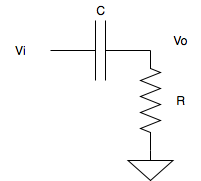
\includegraphics[width=6cm,height=6cm,keepaspectratio]{../Imagenes/CR.png}
	\caption{Filtro pasa altos CR}
	\label{cr}
\end{figure}

\begin{table}[H] 
	\centering
	\begin{tabular}{c c}
		Componentes \\
		\hline
		$R (\Omega)$ & 10k  \\
		$C (F)$ & 1n \\
		\hline
	\end{tabular}
	\caption{Valores elegidos para los componentes de la primera etapa.}
	\label{componentes1}
\end{table}

\subsubsection{Segunda etapa: Filtro pasa altos - Sallen-Key}

 \begin{figure}[H] %!ht
	\centering
	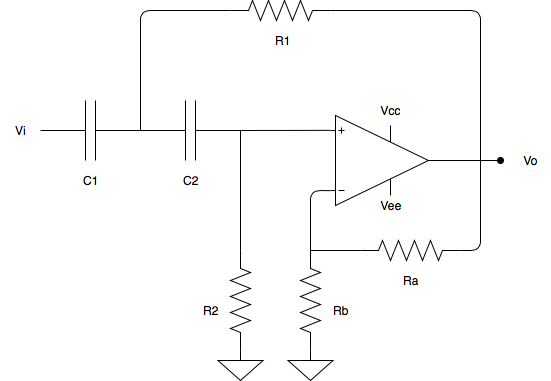
\includegraphics[width=10cm,height=10cm,keepaspectratio]{../Imagenes/sk.png}
	\caption{Filtro pasa altos con celda Sallen-Key}
	\label{sk}
\end{figure}

Los valores de los componentes elegidos para esta etapa, correpsondientes a la figura \ref{sk} y a los valores de Q y de frecuencias de polos y ceros de la tabla \ref{pyc} son los siguientes:

\begin{table}[H] 
	\centering
	\begin{tabular}{c c}
		Componentes \\
		\hline
		$Ra (\Omega)$ &  10k \\
		$Rb (\Omega)$ & 24,23k\\
		$R1 (\Omega)$ &  5,38 \\
		$R2 (\Omega)$ &  5,38 \\
		$C1 (F)$ & 1n \\
		$C2 (F)$ & 1n \\
		\hline
	\end{tabular}
	\caption{Valores elegidos para los componentes de la segunda etapa.}
	\label{componentes2}
\end{table}

Para todas las celdas Sallen-Key se eligieron los componentes mediante el m\'etodo de componentes iguales.

\subsubsection{Tercera etapa: Filtro pasa altos - Sallen-Key}

Los valores para esta celda correspondientes a la imagen \ref{sk} son los siguientes:

\begin{table}[H] 
	\centering
	\begin{tabular}{c c}
		Componentes \\
		\hline
		$Ra (\Omega)$ &  10k \\
		$Rb (\Omega)$ & 10k  \\
		$R1 (\Omega)$ &  7,35 \\
		$R2 (\Omega)$ &  7,35 \\
		$C1 (F)$ & 1n \\
		$C2 (F)$ & 1n \\
		\hline
	\end{tabular}
	\caption{Valores elegidos para los componentes de la tercera etapa.}
	\label{componentes3}
\end{table}

\subsubsection{Cuarta etapa: Filtro pasa altos - Sallen-Key}

Los valores para esta celda correspondientes a la imagen \ref{sk} son los siguientes:

\begin{table}[H] 
	\centering
	\begin{tabular}{c c}
		Componentes \\
		\hline
		$Ra (\Omega)$ &  10k \\
		$Rb (\Omega)$ & 7,17k  \\
		$R1 (\Omega)$ &  9,36 \\
		$R2 (\Omega)$ &  9,36 \\
		$C1 (F)$ & 1n \\
		$C2 (F)$ & 1n \\
		\hline
	\end{tabular}
	\caption{Valores elegidos para los componentes de la cuarta etapa.}
	\label{componentes4}
\end{table}

\subsubsection{Quinta etapa: Filtro pasa altos - Sallen-Key}

Los valores para esta celda correspondientes a la imagen \ref{sk} son los siguientes:

\begin{table}[H] 
	\centering
	\begin{tabular}{c c}
		Componentes \\
		\hline
		$Ra (\Omega)$ &  10k \\
		$Rb (\Omega)$ & 5,95k  \\
		$R1 (\Omega)$ &  10,94 \\
		$R2 (\Omega)$ &  10,94 \\
		$C1 (F)$ & 1n \\
		$C2 (F)$ & 1n \\
		\hline
	\end{tabular}
	\caption{Valores elegidos para los componentes de la quinta etapa.}
	\label{componentes5}
\end{table}

\subsubsection{Sexta etapa: Filtro pasa altos - Flesicher-Tow}


 \begin{figure}[H] %!ht
	\centering
	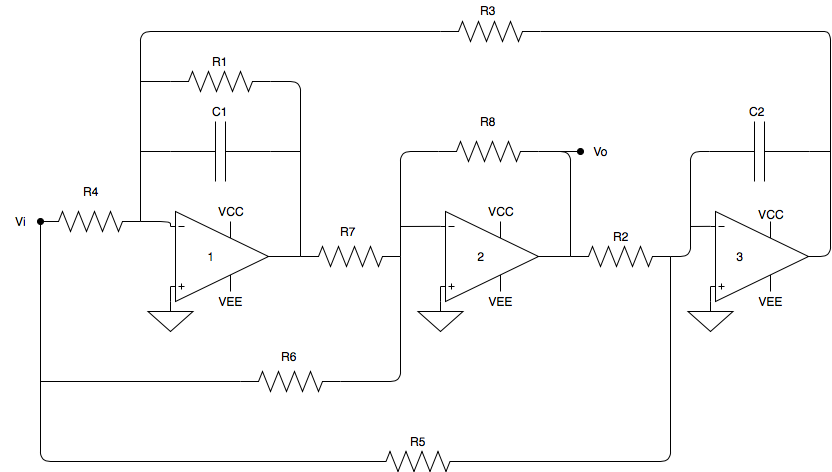
\includegraphics[width=12cm,height=12cm,keepaspectratio]{../Imagenes/FLEISCHER.png}
	\caption{Celda Fleischer-Tow}
	\label{fleischer}
\end{figure}

Los valores para esta celda correspondientes a la imagen \ref{flesicher} son los siguientes:

\begin{table}[H] 
	\centering
	\begin{tabular}{c c}
		Componentes \\
		\hline
		$R1 (\Omega)$ &   \\
		$R2 (\Omega)$ &   \\
		$R3 (\Omega)$ &   \\
		$R4 (\Omega)$ &   \\
		$R5 (\Omega)$ &   \\
		$R6 (\Omega)$ &   \\
		$R7 (\Omega)$ &   \\
		$R8 (\Omega)$ &   \\
		$C1 (F)$ &  \\
		$C2 (F)$ &  \\
		\hline
	\end{tabular}
	\caption{Valores elegidos para los componentes de la sexta etapa.}
	\label{componentes6}
\end{table}

\section{Simulaciones y verificaci\'on}

\section{Mediciones y resultados obtenidos}

\section{Conclusiones}